\scnsegmentheader{Предметная область и онтология субъектно-объектных спецификаций воздействий}

\scnstartsubstruct

\scnrelfromlist{соавтор}{Гордей А.Н.;Никифоров С.А.;Бобёр Е.С.;Святощик М.И.}

\scniselement{предметная область и онтология}

\scnheader{индивид}
\scnidtftext{часто используемый sc-идентификатор}{субъект}
	\scnaddlevel{1}
	\scnrelfrom{источник}{\scncite{Hardzei2005}}
	\scnaddlevel{-1}
	
\scnheader{участник воздействия\scnrolesign}
\scnidtf{участник акции\scnrolesign}
\scniselement{ролевое отношение}
\scnrelfrom{первый домен}{индивид}
\scnrelfrom{второй домен}{воздействие}
\scnexplanation{\textit{участник акции\scnrolesign} -- это ролевое отношение, которое связывает акцию с участвующим в ней индивидом.}
\scnaddlevel{1}
\scnrelfrom{источник}{\scncite{Hardzei2021}}
\scnrelfrom{источник}{\scncite{Fillmore1977}}
\scnrelfrom{источник}{\scncite{Fillmore1982}}
\scnaddlevel{-1}
\scnsubdividing{
	субъект\scnrolesign\\
	\scnaddlevel{1}
	\scnexplanation{\textit{субъект\scnrolesign} -- инициатор акции.}
	\scnsubdividing{
		инициатор\scnrolesign\\
		;вдохновитель\scnrolesign\\	
		;распространитель\scnrolesign\\
		;вершитель\scnrolesign\\
		\scnaddlevel{1}
		\scnexplanation{\textit{вершитель\scnrolesign} завершает акцию производством из объекта продукта.}
		\scnaddlevel{-1}
	}
	\scnaddlevel{-1}
	;инструмент\scnrolesign\\
	\scnaddlevel{1}
	\scnexplanation{\textit{инструмент\scnrolesign} -- исполнитель акции.}
	\scnsubdividing{
		активатор\scnrolesign\\
		\scnaddlevel{1}
		\scnexplanation{\textit{активатор\scnrolesign} непосредственно воздействует на медиатор.}
		\scnaddlevel{-1}
		;супрессор\scnrolesign\\
		\scnaddlevel{1}
		\scnexplanation{\textit{супрессор\scnrolesign} подавляет сопротивление медиатора.}
		\scnaddlevel{-1}
		;усилитель\scnrolesign\\
		\scnaddlevel{1}
		\scnexplanation{\textit{усилитель\scnrolesign} наращивает воздействие на медиатор.}
		\scnaddlevel{-1}
		;преобразователь\scnrolesign\\
		\scnaddlevel{1}
		\scnexplanation{\textit{преобразователь\scnrolesign} преобразует медиатор в инструмент.}
		\scnaddlevel{-1}
	}
	\scnaddlevel{-1}
	;медиатор\scnrolesign\\
	\scnaddlevel{1}
	\scnexplanation{\textit{медиатор\scnrolesign} -- посредник акции.}
	\scnsubdividing{
		ориентир\scnrolesign\\
		;локус\scnrolesign\\
		\scnaddlevel{1}
		\scnexplanation{\textit{локус\scnrolesign} частично или полностью окружает объект и тем самым локализует его в пространстве.}
		\scnaddlevel{-1}
		;транспортёр\scnrolesign\\
		\scnaddlevel{1}
		\scnexplanation{\textit{транспортёр\scnrolesign} перемещает объект.}
		\scnaddlevel{-1}
		;адаптер\scnrolesign\\
		\scnaddlevel{1}
		\scnexplanation{\textit{адаптер\scnrolesign} приспосабливает  инструмент к воздействию на объект.}
		\scnaddlevel{-1}
		;материал\scnrolesign\\
		\scnaddlevel{1}
		\scnexplanation{\textit{материал\scnrolesign} используется в качестве объекта-сырья для производства продукта.}
		\scnaddlevel{-1}
		;макет\scnrolesign\\
		\scnaddlevel{1}
		\scnexplanation{\textit{макет\scnrolesign} является исходным образцом для производства из объекта продукта.}
		\scnaddlevel{-1}
		;фиксатор\scnrolesign\\
		\scnaddlevel{1}
		\scnexplanation{\textit{фиксатор\scnrolesign} превращает переменный локус объекта в постоянный.}
		\scnaddlevel{-1}
		;ресурс\scnrolesign\\
		\scnaddlevel{1}
		\scnexplanation{\textit{ресурс\scnrolesign} питает инструмент.}
		\scnaddlevel{-1}
		;стимул\scnrolesign\\
		\scnaddlevel{1}
		\scnexplanation{\textit{стимул\scnrolesign} проявляет параметр объекта.}
		\scnaddlevel{-1}
		;регулятор\scnrolesign\\
		\scnaddlevel{1}
		\scnexplanation{\textit{регулятор\scnrolesign} служит инструкцией в производстве из объекта продукта.}
		\scnaddlevel{-1}
		;хронотоп\scnrolesign\\
		\scnaddlevel{1}
		\scnexplanation{\textit{хронотоп\scnrolesign} локализует объект во времени.}
		\scnaddlevel{-1}
		;источник\scnrolesign\\
		\scnaddlevel{1}
		\scnexplanation{\textit{источник\scnrolesign} обеспечивает инструкциями инструмент.}
		\scnaddlevel{-1}
		;индикатор\scnrolesign\\
		\scnaddlevel{1}
		\scnexplanation{\textit{индикатор\scnrolesign} отображает параметр воздействия на объект или параметр продукта как результата воздействия на объект.}
		\scnaddlevel{-1}
	}
	\scnaddlevel{-1}
	;объект\scnrolesign\\
	\scnaddlevel{1}
	\scnexplanation{\textit{объект\scnrolesign} -- реципиент акции.}
	\scnsubdividing{
		покрытие\scnrolesign\\
		\scnaddlevel{1}
		\scnexplanation{\textit{покрытие\scnrolesign} -- внешняя изоляция оболочки индивида.}
		\scnaddlevel{-1}
		;корпус\scnrolesign\\
		\scnaddlevel{1}
		\scnexplanation{\textit{корпус\scnrolesign} -- оболочка индивида.}
		\scnaddlevel{-1}
		;прослойка\scnrolesign\\
		\scnaddlevel{1}
		\scnexplanation{\textit{прослойка\scnrolesign} -- внутренняя изоляция оболочки индивида.}
		\scnaddlevel{-1}
		;сердцевина\scnrolesign\\
		\scnaddlevel{1}
		\scnexplanation{\textit{сердцевина\scnrolesign} -- ядро индивида.}
		\scnaddlevel{-1}
	}
	\scnaddlevel{-1}
	;продукт\scnrolesign\\
	\scnaddlevel{1}
	\scnexplanation{\textit{продукт\scnrolesign} -- результат воздействия субъекта на объект.}
	\scnsubdividing{
		заготовка\scnrolesign\\
		\scnaddlevel{1}
		\scnexplanation{\textit{заготовка\scnrolesign} -- превращённый в сырьё объект.}
		\scnaddlevel{-1}
		;полуфабрикат\scnrolesign\\
		\scnaddlevel{1}
		\scnexplanation{\textit{полуфабрикат\scnrolesign} -- наполовину изготовленный из сырья продукт.}
		\scnaddlevel{-1}
		;прототип\scnrolesign\\
		\scnaddlevel{1}
		\scnexplanation{\textit{прототип\scnrolesign} -- опытный образец продукта.}
		\scnaddlevel{-1}
		;изделие\scnrolesign\\
		\scnaddlevel{1}
		\scnexplanation{\textit{изделие\scnrolesign} -- готовый продукт.}
		\scnaddlevel{-1}
	}
	\scnaddlevel{-1}
}

\scnheader{воздействие}
\scnidtf{акция}
\scnrelfrom{источник}{\scncite{Hardzei2017}}
\scnrelfrom{разбиение}{\scnkeyword{Типология по характеру взаимодействия участников\scnsupergroupsign}}
\scnaddlevel{1}
\scneqtoset{
	воздействие активизации\\
	\scnaddlevel{1}
	\scnexplanation{\textit{воздействие активизации} -- воздействие, в ходе которого взаимодействие осуществляется между субъектом и инструментом.}
	\scnaddlevel{-1}
	;воздействие эксплуатации\\
	\scnaddlevel{1}
	\scnexplanation{\textit{воздействие эксплуатации} -- воздействие, в ходе которого взаимодействие осуществляется между инструментом и медиатором.}
	\scnaddlevel{-1}
	;воздействие трансформации\\
	\scnaddlevel{1}
	\scnexplanation{\textit{воздействие трансформации} -- воздействие, в ходе которого взаимодействие осуществляется между объектом и продуктом.}
	\scnaddlevel{-1}
	;воздействие нормализации\\
	\scnaddlevel{1}
	\scnexplanation{\textit{воздействие нормализации} -- воздействие, в ходе которого взаимодействие осуществляется между объектом и продуктом.}
	\scnaddlevel{-1}
}
\scnaddlevel{-1}
\scnrelfrom{разбиение}{\scnkeyword{Типология воздействий по виду взаимодействующих подсистем\scnsupergroupsign}}
\scnaddlevel{1}
\scneqtoset{
	воздействие среда-оболочка\\
	;воздействие оболочка-ядро\\
	;воздействие ядро-оболочка\\
	;воздействие оболочка-среда
}

\scnheader{воздействие}
\scnrelfrom{разбиение}{\scnkeyword{Типология воздействий по фазам наращивания воздействия\scnsupergroupsign}}
\scnaddlevel{1}
\scneqtoset{
	воздействие инициации\\
	\scnaddlevel{1}
	\scnexplanation{\textit{воздействие инициации} -- воздействие, в ходе которого оно начинается в каждой подсистеме.}
	\scnaddlevel{-1}
	;воздействие аккумуляции\\
	\scnaddlevel{1}
	\scnexplanation{\textit{воздействие аккумуляции} -- воздействие, в ходе которого происходит его накапливание в каждой подсистеме.}
	\scnaddlevel{-1}
	;воздействие амплификации\\
	\scnaddlevel{1}
	\scnexplanation{\textit{воздействие амплификации} -- воздействие, в ходе которого происходит его усиление.}
	\scnaddlevel{-1}
	;воздействие генерации\\
	\scnaddlevel{1}
	\scnexplanation{\textit{воздействие генерации} -- воздействие, которое представляет собой переход в каждой подсистеме с одного уровня, например, среды-оболочки, на другой, например, оболочки-ядра.}
	\scnaddlevel{-1}
}
\scnaddlevel{-1}

\scnheader{воздействие}
\scnrelfrom{разбиение}{\scnkeyword{Типология воздействий по виду инструмента\scnsupergroupsign}}
\scnaddlevel{1}
\scneqtoset{
	физическое воздействие\\
	\scnaddlevel{1}
	\scnexplanation{\textit{физическое воздействие} -- воздействие, в котором в роли инструмента выступает оболочка субъекта.}
	\scnaddlevel{-1}	
	;информационное воздействие\\
	\scnaddlevel{1}
	\scnexplanation{\textit{информационное воздействие} -- воздействие, в котором в роли инструмента выступает среда субъекта.}
	\scnaddlevel{-1}
}
\scnaddlevel{-1}

\scnheader{Рис. Таблица воздействий}
\scneqfile{\\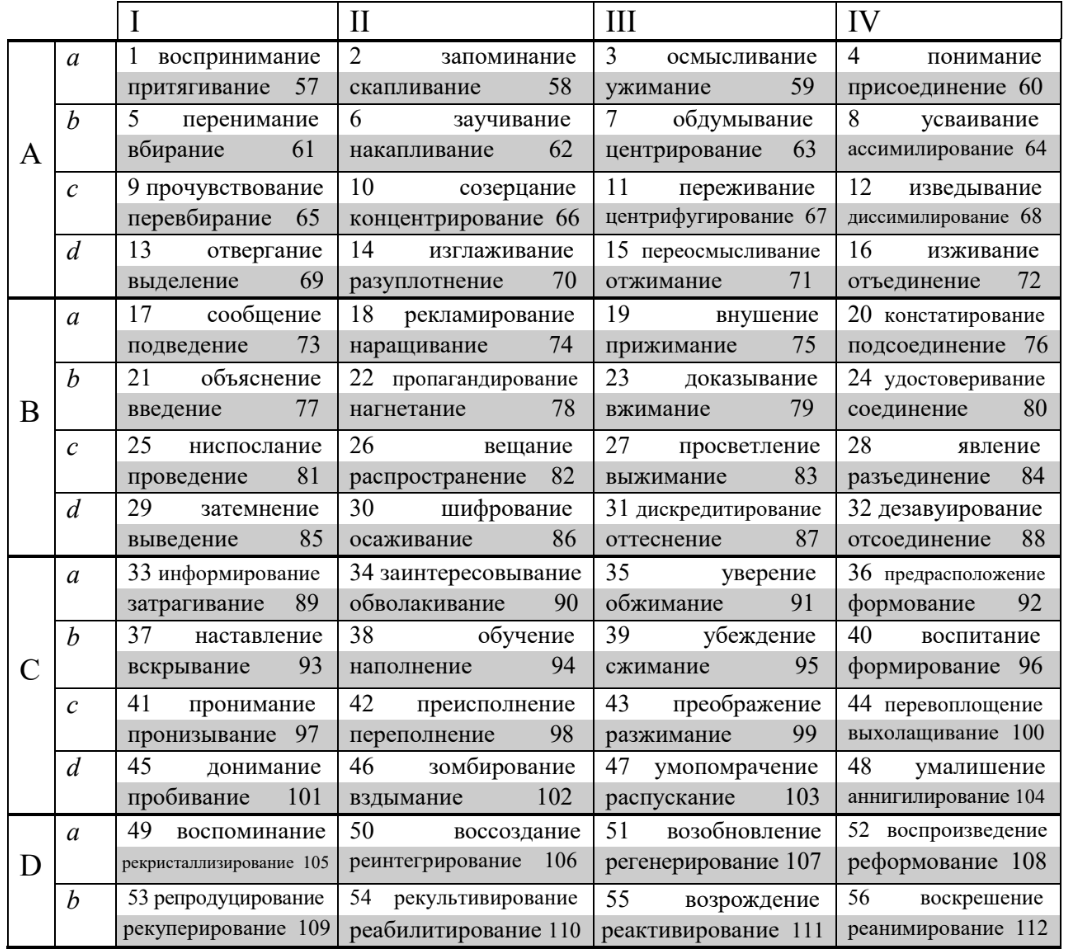
\includegraphics[width=0.9\linewidth]{figures/sd_actions/macroproc_table.png}\\}
\scnrelfrom{источник}{\scncite{Hardzei2017}}
\scnexplanation{На изображении представлена типология \textit{воздействий}. Любое воздействие характеризуется принадлежностью четырём классам, соответствующим признакам классификации. Заштрихованы \textit{физические воздействия}.}

\scnheader{Специфицируемые классы воздействий}
\scnsuperset{
	\scnmakesetlocal{
		формование\\
		\scnaddlevel{1}
		\scnreltoset{пересечение}{воздействие трансформации;воздействие среда-оболочка;воздействие генерации;физическое воздействие}
		\scnaddlevel{-1}
		;притягивание\\
		\scnaddlevel{1}
		\scnreltoset{пересечение}{воздействие активизации;воздействие среда-оболочка;воздействие инициации;физическое воздействие}
		\scnaddlevel{-1}
		;выхолащивание\\
		\scnaddlevel{1}
		\scnreltoset{пересечение}{воздействие трансформации;воздействие ядро-оболочка;воздействие генерации;физическое воздействие}
		\scnaddlevel{-1}
		;аннигилирование\\
		\scnaddlevel{1}
		\scnreltoset{пересечение}{воздействие трансформации;воздействие оболочка-среда;воздействие генерации;физическое воздействие}
		\scnaddlevel{-1}
		;введение\\
		\scnaddlevel{1}
		\scnreltoset{пересечение}{воздействие эксплуатации;воздействие оболочка-ядро;воздействие инициации;физическое воздействие}
		\scnaddlevel{-1}
		;распускание\\
		\scnaddlevel{1}
		\scnreltoset{пересечение}{воздействие трансформации;воздействие оболочка-среда;воздействие амплификации;физическое воздействие}
		\scnaddlevel{-1}
		;разжимание\\
		\scnaddlevel{1}
		\scnreltoset{пересечение}{воздействие трансформации;воздействие ядро-оболочка;воздействие амплификации;физическое воздействие}
		\scnaddlevel{-1}
		;разъединение\\
		\scnaddlevel{1}
		\scnreltoset{пересечение}{воздействие эксплуатации;воздействие ядро-оболочка;воздействие генерации;физическое воздействие}
		\scnaddlevel{-1}
	}
}

\scnheader{Пример sc.g-текста, описывающего спецификацию воздействия}
\scneqscg{figures/sd_actions/tapaz_description_example.png}
\scniselement{sc.g-текст}
\scnexplanation{Представленный фрагмент базы знаний содержит декомпозицию воздействия во времени, указание принадлежности данного декомпозируемого воздействия и полученных в результате данной декомпозиции воздействий определенному их классу из приведенной выше классификации, а также указание участников данных акций.}
\scnexplanation{Представленный фрагмент базы знаний можно протранслировать в следующий текст естественного языка: <<Некто принимает молоко, затем окисляет молоко, а именно: нормализует молоко до 15-процентной жирности, затем очищает молоко, затем пастеризует молоко, затем охлаждает молоко до определённой температуры, затем вносит закваску в молоко, затем сквашивает молоко, затем режет сгусток, затем подогревает сгусток, затем обрабатывает сгусток, затем отделяет сыворотку, затем охлаждает сгусток и, в итоге, производит творог>>.}

\scnheader{субъект}
\scnidtftext{часто используемый sc-идентификатор}{индивид}
\scnidtf{активная сущность}
\scnidtf{сущность, способная самостоятельно выполнять некоторые виды действий}
\scnidtf{агент деятельности}
\scnsuperset{Собственное Я}
\scnsuperset{внутренний субъект ostis-системы}
\scnsuperset{внешний субъект ostis-системы, с которым осуществляется взаимодействие}
\scnsuperset{внешний субъект ostis-системы, с которым взаимодействие не происходит}

\scnheader{внутренний субъект ostis-системы}
\scnidtf{субъект, входящий в состав той \textit{ostis-системы, в базе знаний} которой он описывается}
\scnsuperset{sc-агент}
\scnexplanation{Под \textit{внутренним субъектом ostis-системы} понимается такой \textit{субъект}, который выполняет некоторые \textit{действия} в \uline{той же памяти}, в которой хранится его знак.
	\newline
	К числу \textit{внутренних субъектов ostis-системы} относятся входящие в нее \textit{sc-агенты}, частные sc-машины, целые интеллектуальные подсистемы.}

\scnheader{внешний субъект ostis-системы, с которым осуществляется взаимодействие}
\scnexplanation{К числу \textit{внешних субъектов ostis-системы, с которыми осуществляется взаимодействие}, относятся конечные пользователи \textit{ostis-системы}, ее разработчики, а также другие компьютерные системы(причем не только интеллектуальные).}

\scnheader{субъект действия\scnrolesign}
\scnsubset{субъект\scnrolesign}
\scnidtf{сущность, воздействующая на некоторую другую сущность в процессе заданного действия\scnrolesign}
\scnidtf{сущность, создающая \textit{причину} изменений другой сущности (объекта действия)\scnrolesign}
\scnidtf{быть субъектом данного действия\scnrolesign}
\scnsuperset{субъект неосознанного воздействия\scnrolesign}
\scnsuperset{субъект осознанного воздействия\scnrolesign}
\scnaddlevel{1}
\scnidtf{субъект целенаправленного, активного воздействия\scnrolesign}
\scnaddlevel{-1}

\scnheader{исполнитель*}
\scnexplanation{Связки отношения \textit{исполнитель*} связывают \textit{sc-элементы}, обозначающие \textit{действие} и \textit{sc-элементы}, обозначающие \textit{субъекта}, который предположительно будет осуществлять, осуществляет или осуществлял выполнение указанного \textit{действия}. Данное отношение может быть использовано при назначении конкретного исполнителя для проектной задачи по развитию баз знаний.
	
	В случае, когда заранее неизвестно, какой именно \textit{субъект*} будет исполнителем данного \textit{действия}, отношение \textit{исполнитель*} может отсутствовать в первоначальной формулировке \textit{задачи} и добавляться позже, уже непосредственно при исполнении.
	
	Когда действие выполняется (является \textit{настоящей сущностью}) или уже выполнено (является \textit{прошлой сущностью}), то исполнитель этого действия в каждый момент времени уже определён. Но когда действие только инициировано, тогда важно знать:
	\begin{enumerate}
		\item кто \uline{хочет} выполнить это действие и насколько важно для него стать исполнителем данного действия;	
		\item кто \uline{может} выполнить данное действие и каков уровень его квалификации и опыта;
		\item кто и кому поручает выполнить это действие и каков уровень ответственности за невыполнение (приказ, заказ, официальный договор, просьба...)
	\end{enumerate}	
	При этом следует помнить, что связь отношения \textit{исполнитель*} в данном случае также является временной прогнозируемой сущностью.
	
	Первым компонентом связок отношений \textit{исполнитель*} является знак \textit{действия}, вторым -- знак \textit{субъекта} исполнителя}

\scnheader{объект воздействия\scnrolesign}
\scnsubset{объект\scnrolesign}
\scnidtf{сущность, на которую осуществляется воздействие в рамках заданного действия\scnrolesign}
\scnidtf{сущность, являющаяся в рамках заданного действия исходным условием (аргументом), необходимым для выполнения этого действия\scnrolesign}
\scnnote{Для разных действий количество объектов действий может быть различным.}
\scnnote{Поскольку действие является процессом и, соответственно, представляет собой \textit{динамическую структуру}, то и знак \textit{субъекта действия\scnrolesign}, и знак \textit{объекта действия\scnrolesign} являются элементами данной структуры. В связи с этим можно рассматривать отношения \textit{субъект действия\scnrolesign} и \textit{объект действия\scnrolesign} как \textit{ролевые отношения}. Данный факт не  запрещает вводить аналогичные \textit{неролевые отношения}, однако это нецелесообразно.}

\scnheader{продукт\scnrolesign}
\scnidtf{быть продуктом заданного действия\scnrolesign}
\scnsubset{продукт*}
\scnsubset{результат*}
\scnidtf{"сухой"{} остаток\scnrolesign
}
\scnidtf{то, ради чего может быть выполнено, выполняется или будет выполняться заданное действие\scnrolesign}
\scnnote{Продуктом действия может быть некоторая материальная сущность, некоторое множество (тираж) одинаковых материальных сущностей, некоторая информационная конструкция}

\scnheader{результат*}
\scnexplanation{Связки отношения \textit{результат*} связывают \textit{sc-элемент}, обозначающий \textit{действие}, и \textit{sc-конструкцию}, описывающую результат выполнения рассматриваемого действия, другими словами, цель, которая должна быть достигнута при выполнении \textit{действия}.
	
	Результат может специфицироваться как атомарным высказыванием, так и неатомарным, т.е. конъюнктивным, дизъюнктивным, строго дизъюнктивным и т.д.
	
	В случае, когда успешное выполнение \textit{действия} приводит к изменению какой-либо конструкции в \textit{\mbox{sc-памяти}}, которое необходимо занести в историю изменений базы знаний или использовать для демонстрации протокола решении задачи, генерируется соответствующая связка отношения \textit{результат*}, связывающая задачу и \textit{sc-конструкцию}, описывающую данное изменение. Конкретный вид указанной \textit{\mbox{sc-конструкции}} зависит от типа действия.}
\scnrelboth{следует отличать}{цель*}
\scnaddlevel{1}
\scnidtf{спецификация планируемого результата*}
\scnnote{Следует также отмечать то, что является непосредственно результатом (продуктом) некоторого действия, и то, что является предварительной (исходной, стартовой) спецификацией этого  результата. Далеко не всегда результатом действия является именно то, что планировалось (было целью) изначально.}
\scnaddlevel{-1}

\scnheader{класс выполняемых действий*}
\scnidtf{класс действий, выполняемых классом субъектов*}
\scnexplanation{Связки отношения \textit{класс выполняемых действий*} связывают классы \textit{субъектов} и классы действий, при этом предполагается, что каждый субъект указанного класса способен выполнять действия указанного класса действий.}

\scnheader{заказчик*}
\scnexplanation{Связки отношения \textit{заказчик*} связывают классы \textit{sc-элементы}, обозначающие \textit{действие}, и \textit{sc-элементы}, обозначающие  \textit{субъекта}, который "заинтересован"{} в выполнении данного действия и, как правило, инициирует его выполнение. Данное отношение может быть использовано при указании того, кто поставил проектную задачу по развитию баз знаний.
	
	Первым компонентов связок отношения \textit{заказчик*} является знак \textit{действия}, вторым -- знак \textit{субъекта}.}

\scnheader{инициатор*}
\scnexplanation{Связки отношения \textit{инициатор*} связывают \textit{sc-элемент}, обозначающий \textit{инициированное действие}, и знак \textit{субъекта}, который является инициатором данного \textit{действия}, то есть \textit{субъектом}, который инициировал данное \textit{действие} и, как правило, заинтересован в его успешном выполнении.}

\scnheader{объект\scnrolesign}
\scnidtf{аргумент действия\scnrolesign}
\scnexplanation{Связки отношения \textit{объект\scnrolesign} связывают \textit{sc-элемент}, обозначающий \textit{действие}, и знак той сущности, над которой (по отношению к которой) осуществляется данное \textit{действие}, и, например, знак \textit{структуры}, подлежащий верификации.}
\scnsuperset{первый аргумент действия\scnrolesign}
\scnsuperset{второй аргумент действия\scnrolesign}
\scnsuperset{третий аргумент действия\scnrolesign}

\scnheader{класс аргументов*}
\scnidtf{класс аргументов класса команд*}
\scnidtf{быть классом sc-элементов, экземпляры которого являются аргументами для заданного класса команд*}
\scnsuperset{класс первых аргументов*}
\scnsuperset{класс вторых аргументов*}
\scnexplanation{Связки отношения \textit{класс аргументов*} связывают \textit{классы команд} (подмножества множества \textit{команд}) и классы \textit{sc-элементов}, которые могут быть аргументами действий, соответствующих данному  \textit{классу команд}. В случае, когда  \textit{команды} данного класса имеют один аргумент, используется собственно отношение  \textit{класс аргументов*}, в случае, когда команды данного класса имеют более одного аргумента, то используются подмножества данного отношения, такие как \textit{класс первых аргументов*}, \textit{класс вторых аргументов*} и т.д.
	
	Если для некоторого \textit{класса команд} не указан тип какого-либо из аргументов, то предполагается, что в качестве данного аргумента может выступать любой \textit{sc-элемент}.
	
	Первым компонентом связок отношения \textit{класс аргументов*} является знак \textit{класса команд}, вторым -- знак класса \textit{sc-элемента}, которые могут быть \textit{аргументами действий\scnrolesign}, соответствующих данному \textit{классу команд}.}

\bigskip

\scnendstruct \scnendsegmentcomment{Предметная область и онтология субъектно-объектных спецификаций воздействий}
